% link for the text :
% http://christopher5106.github.io/deep/learning/2016/09/16/about-loss-functions-multinomial-logistic-logarithm-cross-entropy-square-errors-euclidian-absolute-frobenius-hinge.html
\documentclass{report}

\usepackage{graphicx}  % package for importing images
\usepackage{mathtools} % package for math equation
\usepackage{mathrsfs}  % package for math font
% \usepackage{amsmath}

\graphicspath{ {./} }
\begin{document}

\chapter {Losses}
A loss is a "penalty" score to reduce when training an algorithm on data. It is usually call \textbf{objective function} to
optimize.

Classifying means assigning a label to an observation:

x $\, \to \,$ y.

Such a function is named a \textbf{classifier}. To create such classifier, we ussually create models with parameters to define:
\[ f_w  : x \to y \]

The process of defining the optimal parameters \textit{w} given past observations X and their known labels Y is named \textbf{training}.
The objective of the training is obviously to maximize the \textbf{likelihood}
\[ likelihood(w) = P_w(y|w) \]

Since the logarithm is monotonous, it is equivalent to \textbf{minimize the negative log-likelihood}
\[ \mathscr{L}( w ) = - \ln P_w( y | x ) \]

The reasons for taking the negative of the logarithm of the likelihood are :
\begin{itemize}
\item it is more convinient to work with the log, because the log-likelihood of statistically independant observations will
  simply be the sum of the log-likelihood of each observation
\item we usually prefer to write the \textbf{objective function} as a \textbf{cost function} to minimize.
\end{itemize}

\section {Binomial probabilities - log loss / logistic loss / cross-entropy loss}

Binomial means 2 classes, which usually are 0 or 1. Each class has a probability \textit{p} and \textit{1-p} (sums to 1).
When using a network, we try to get 0 and 1 as values, that's why we add a \textbf{sigmoid function or logistic function} that saturates
as a last layer.

% for adding image

\[  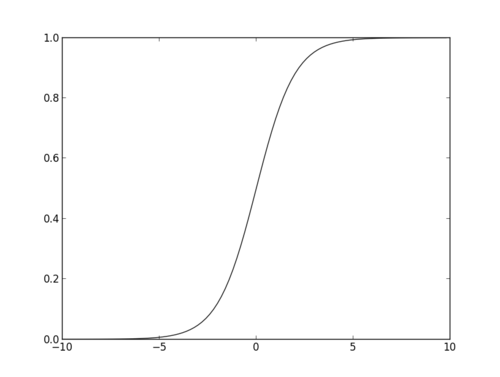
\includegraphics[scale=0.7]{sigmoid} \]
\[ f:  x \rightarrow \frac{1}{ 1 + e^{-x}} \]

Then, once the estimated probability to get 1 is \^{p}, then it is easy to see that the negative log likelihood can be written
\[ \mathscr{L} = - y \log \hat{p}  - (1 - y) \log ( 1 - \hat{p} ) \]

which is also the \textbf{cross-entropy}
\[\text{crossentropy} (p , q ) = E_p [ -\log q ] = - \sum_x p(x ) \log q(x) = - \frac{1}{N} \sum_{n=1}^N \log q(x_n) \]

\section {Multinomial probabilities / multi-class classification : multinomial logistic loss / cross entropy loss / log loss}

It is a problem where we have \textit{k} classes or categories, and only one valid for each example.
The target values are still binary but represented as a vector y that will be defined  by the following, if the example x is of class c:
\[
  y_i = 
\begin{cases}
  0, & \text{ if } i \neq  c \\
  1, & \text{ otherwise }
\end{cases}
\]

If \{pi\} is the probability of each class, then it is a multinomial distribution and
\[ \sum_i p_i = 1\]

The equivalent to the sigmoid functoin in multi-dimensional space is the \textbf{softmax function or logistic function or normalized
  exponential function} to produce such a distribution from any input vector \textit{z} :
\[ z \rightarrow \left\{ \frac{\exp z_i }{ \sum_k \exp^{z_k} } \right\}_i \]

The error is also best described by cross-entropy :
\[ \mathscr{L} = - \sum_{i=0}^k y_i \ln \hat{p}_i \]

Cross-entropy is designed to deal with error on probabilities. For example, ln(0,01) will be a lot stronger error signal than ln(0.1)
and encourage to resolve errors. In some cases, the logarithm is bounded to avoid extreme punishments.

Last, the combined softmax and cross-entropy has a very simple and stable derivative.

\section{Multi-label classification}

There is a variant for multi-label classification, in this case multiple $y_i$ can have a value set to 1. For example, "car", "automobile",
"motor vehicle" are three labels that can be applied to a same image of a car. On the image of a truck, you'll only have "motor vehicle"
active for example. In this case, the softmax function will not apply, we usually add a sigmoïd layer before the cross-entropy layer to ensure stable gradient estimation :
\[ t \rightarrow \frac{1}{1+e^{-t}} \]

The cross-entropy will look like :
\[ \mathscr{L} = - \sum_{i=0}^k y_i \ln \hat{p}_i + (1 - y_i) \ln ( 1 - \hat{p}_i ) \]


\section{Absolute value loss / L1 loss}

The absolute value los is the L1-norm of the error :
\[ \mathscr{L}_1 = \sum_i |  \hat{y}_i - y_i | = \| \hat{y} - y \|_1 \]

Minimizing the absolute value loss means predicting the (conditional) median of \textit{y}. Variants can handle other quantiles. 0/1 loss
for classification is a special case.
Note that the L1 norm is not differentable in 0, and it is possible to use a smooth L1:
\[
\lvert{ d } \rvert_{\text{smooth}} ==   \begin{cases}
   0.5 d^2, & \text{if}\ | d  | \leq 1 \\
   | d | - 0.5, & \text{otherwise}
 \end{cases}
\]

\section {L2 Loss }
When predictions are scalars or metrics we usually use the \textbf{square error or euclidean loss} which is the L2-norm of the error:
\[ \mathscr{L}_2 = \sum_i {(  \hat{y}_i - y_i )}^2 = \| \hat{y} - y \|_2^2 \]

Minimising the squared error is equivalent to predicting the (conditional) mean of y. Due to the gradient being flat at the extremes for
a sigmoid function, we do not use a sigmoid activation with a squared error loss because convergence will be slow if some neurons saturate
on the wrong side.

A squared error is often used with a rectified linear unit. The L2 norm penalizes large errors more strongly and therefore is very sensitive to outliers. To avoid this, we usually use the squared root version :
\[ \mathscr{L} = \| \hat{y} - y \|_2 \]
\end{document}
